\chapter{DOMAIN ANALYSIS}

\section{Problem Definition \& Analysis}

This section establishes the problem addressed by the present work and analyses it across four complementary dimensions: epidemiological burden, biomechanical load, accessibility mismatch, and interaction-bandwidth constraint. Each dimension is examined with reference to peer-reviewed evidence, with the objective of demonstrating that classical computer input methods produce a measurable ergonomic and inclusion gap that justifies investigation of a wearable, movement-native alternative. The chapter concludes with a formal problem statement that synthesises the findings of the analysis.

\subsection{Problem Definition}

Classical computer input devices, particularly mice and trackpads, remain the dominant interaction mechanism in office, educational, and home-computing contexts. Their performance advantages for precision pointing are well established; however, they rely on prolonged static postures, repetitive micro-movements, and environmentally constrained fine-motor control. These properties increasingly conflict with contemporary computing patterns, where users interact for longer durations, in more diverse physical contexts, and with more heterogeneous physical abilities.

The long-horizon trajectory of this burden is summarised in Figure~\ref{fig:msd_global_trend}, which shows the growth in global prevalence estimates and projections.
\begin{figure}[ht!]
  \centering
  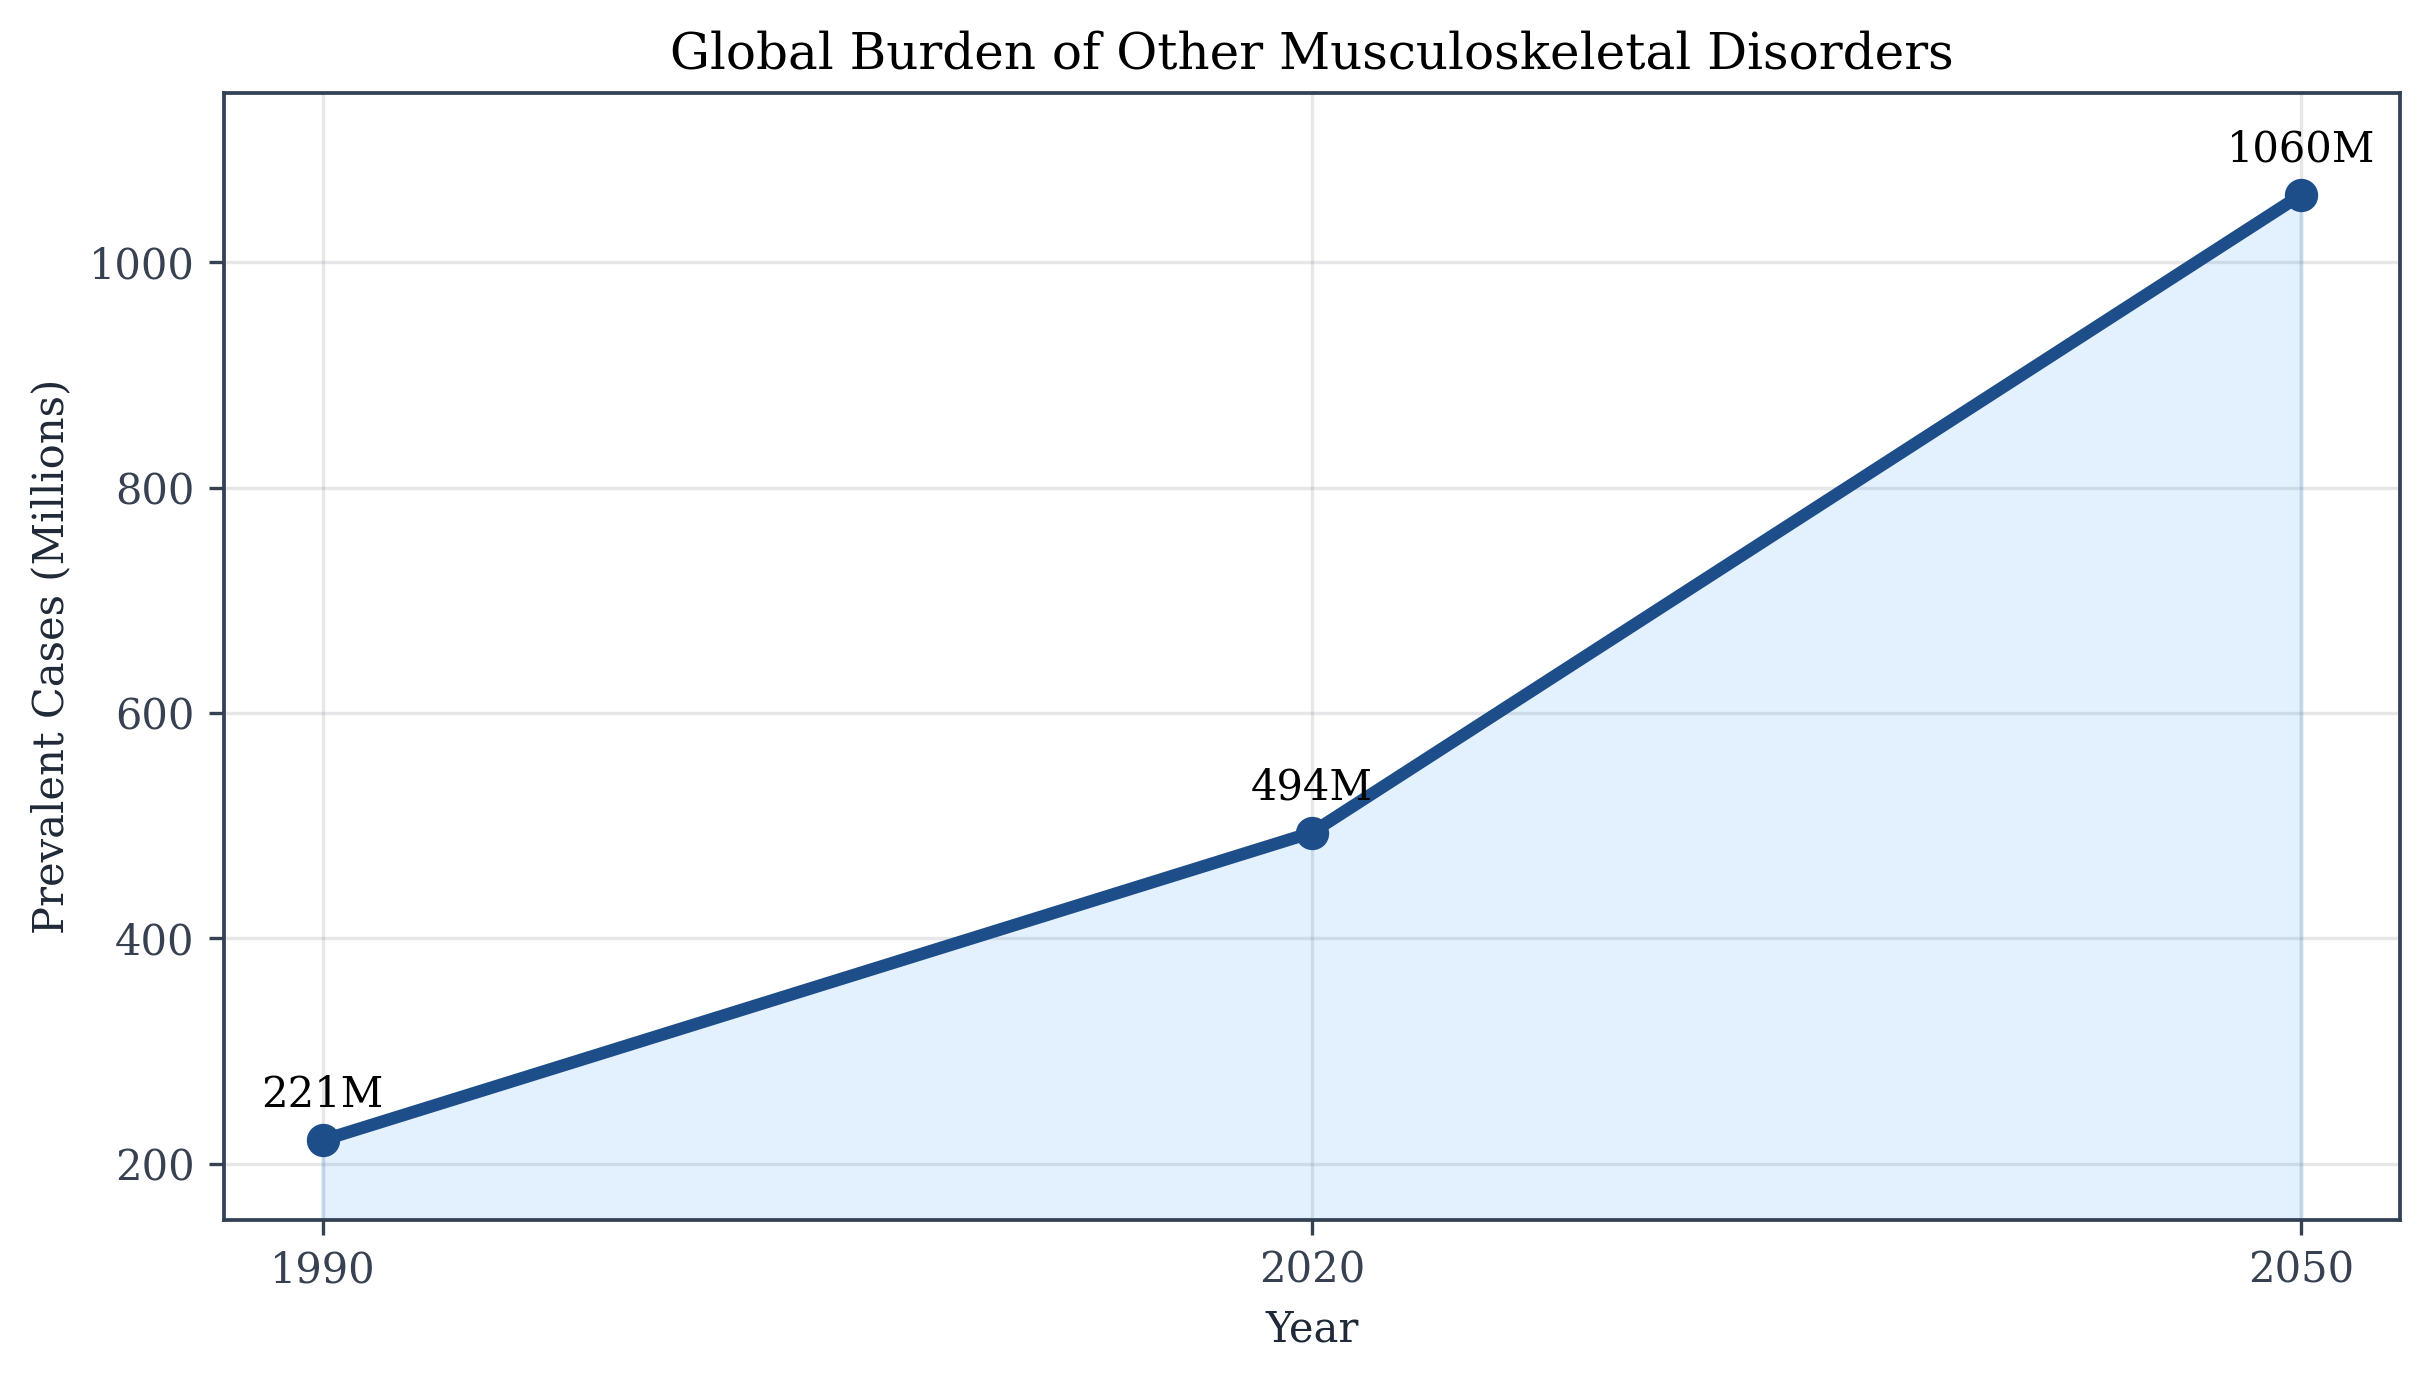
\includegraphics[width=0.7\linewidth]{img/ch1_msd_burden_trend.png}
  \caption{Global Growth in Other Musculoskeletal Disorder Cases (1990--2050 Projection)}
  \label{fig:msd_global_trend}
\end{figure}

Therefore, the core problem is not only discomfort at the individual level, but a systemic mismatch between the assumptions embedded in classical input devices and the current human, clinical, and contextual realities of computer use.

\newpage
The health burden associated with this interaction model is substantial. A systematic review found work-related musculoskeletal disorder (MSD) prevalence among computer users ranging from 33.8\% to 95.3\% depending on cohort and diagnostic approach~\cite{demissie2024wrmsd}. At population scale, the burden is amplified: musculoskeletal conditions affect approximately 1.71~billion people globally~\cite{who2022musculoskeletal}, and disability affects roughly 1.3~billion people~\cite{who2022disability}. Long-term trend data indicate that this is not a static issue; the Global Burden of Disease analysis reports a 123.4\% increase in MSD cases from 1990--2020, with projections continuing upward to 2050~\cite{gbd2023othermsd}.

\subsection{Problem Analysis}

The causes and impacts of the identified problem are multifactorial and can be analysed across four dimensions: biomechanical load, accessibility mismatch, environmental dependency, and interaction-bandwidth limitation.

\subsubsection{Biomechanical Load and Injury Risk}

Biomechanical studies identify several concurrent stressors during classical mouse use: forearm pronation, wrist extension, static muscular activation, and repetitive click-force execution. In controlled comparisons, classical mouse posture requires approximately 42$^\circ$ of forearm pronation, while alternative ergonomic configurations reduce this value and the associated extensor-muscle activation~\cite{quemelo2013vertical}. Wrist extension commonly exceeds 30$^\circ$ across multiple device designs~\cite{feathers2013alternative}, and carpal-tunnel pressure in symptomatic users has been measured at levels substantially above established neurophysiological risk thresholds during mousing tasks~\cite{schmid2015vertical}.
\begin{figure}[H]
  \centering
  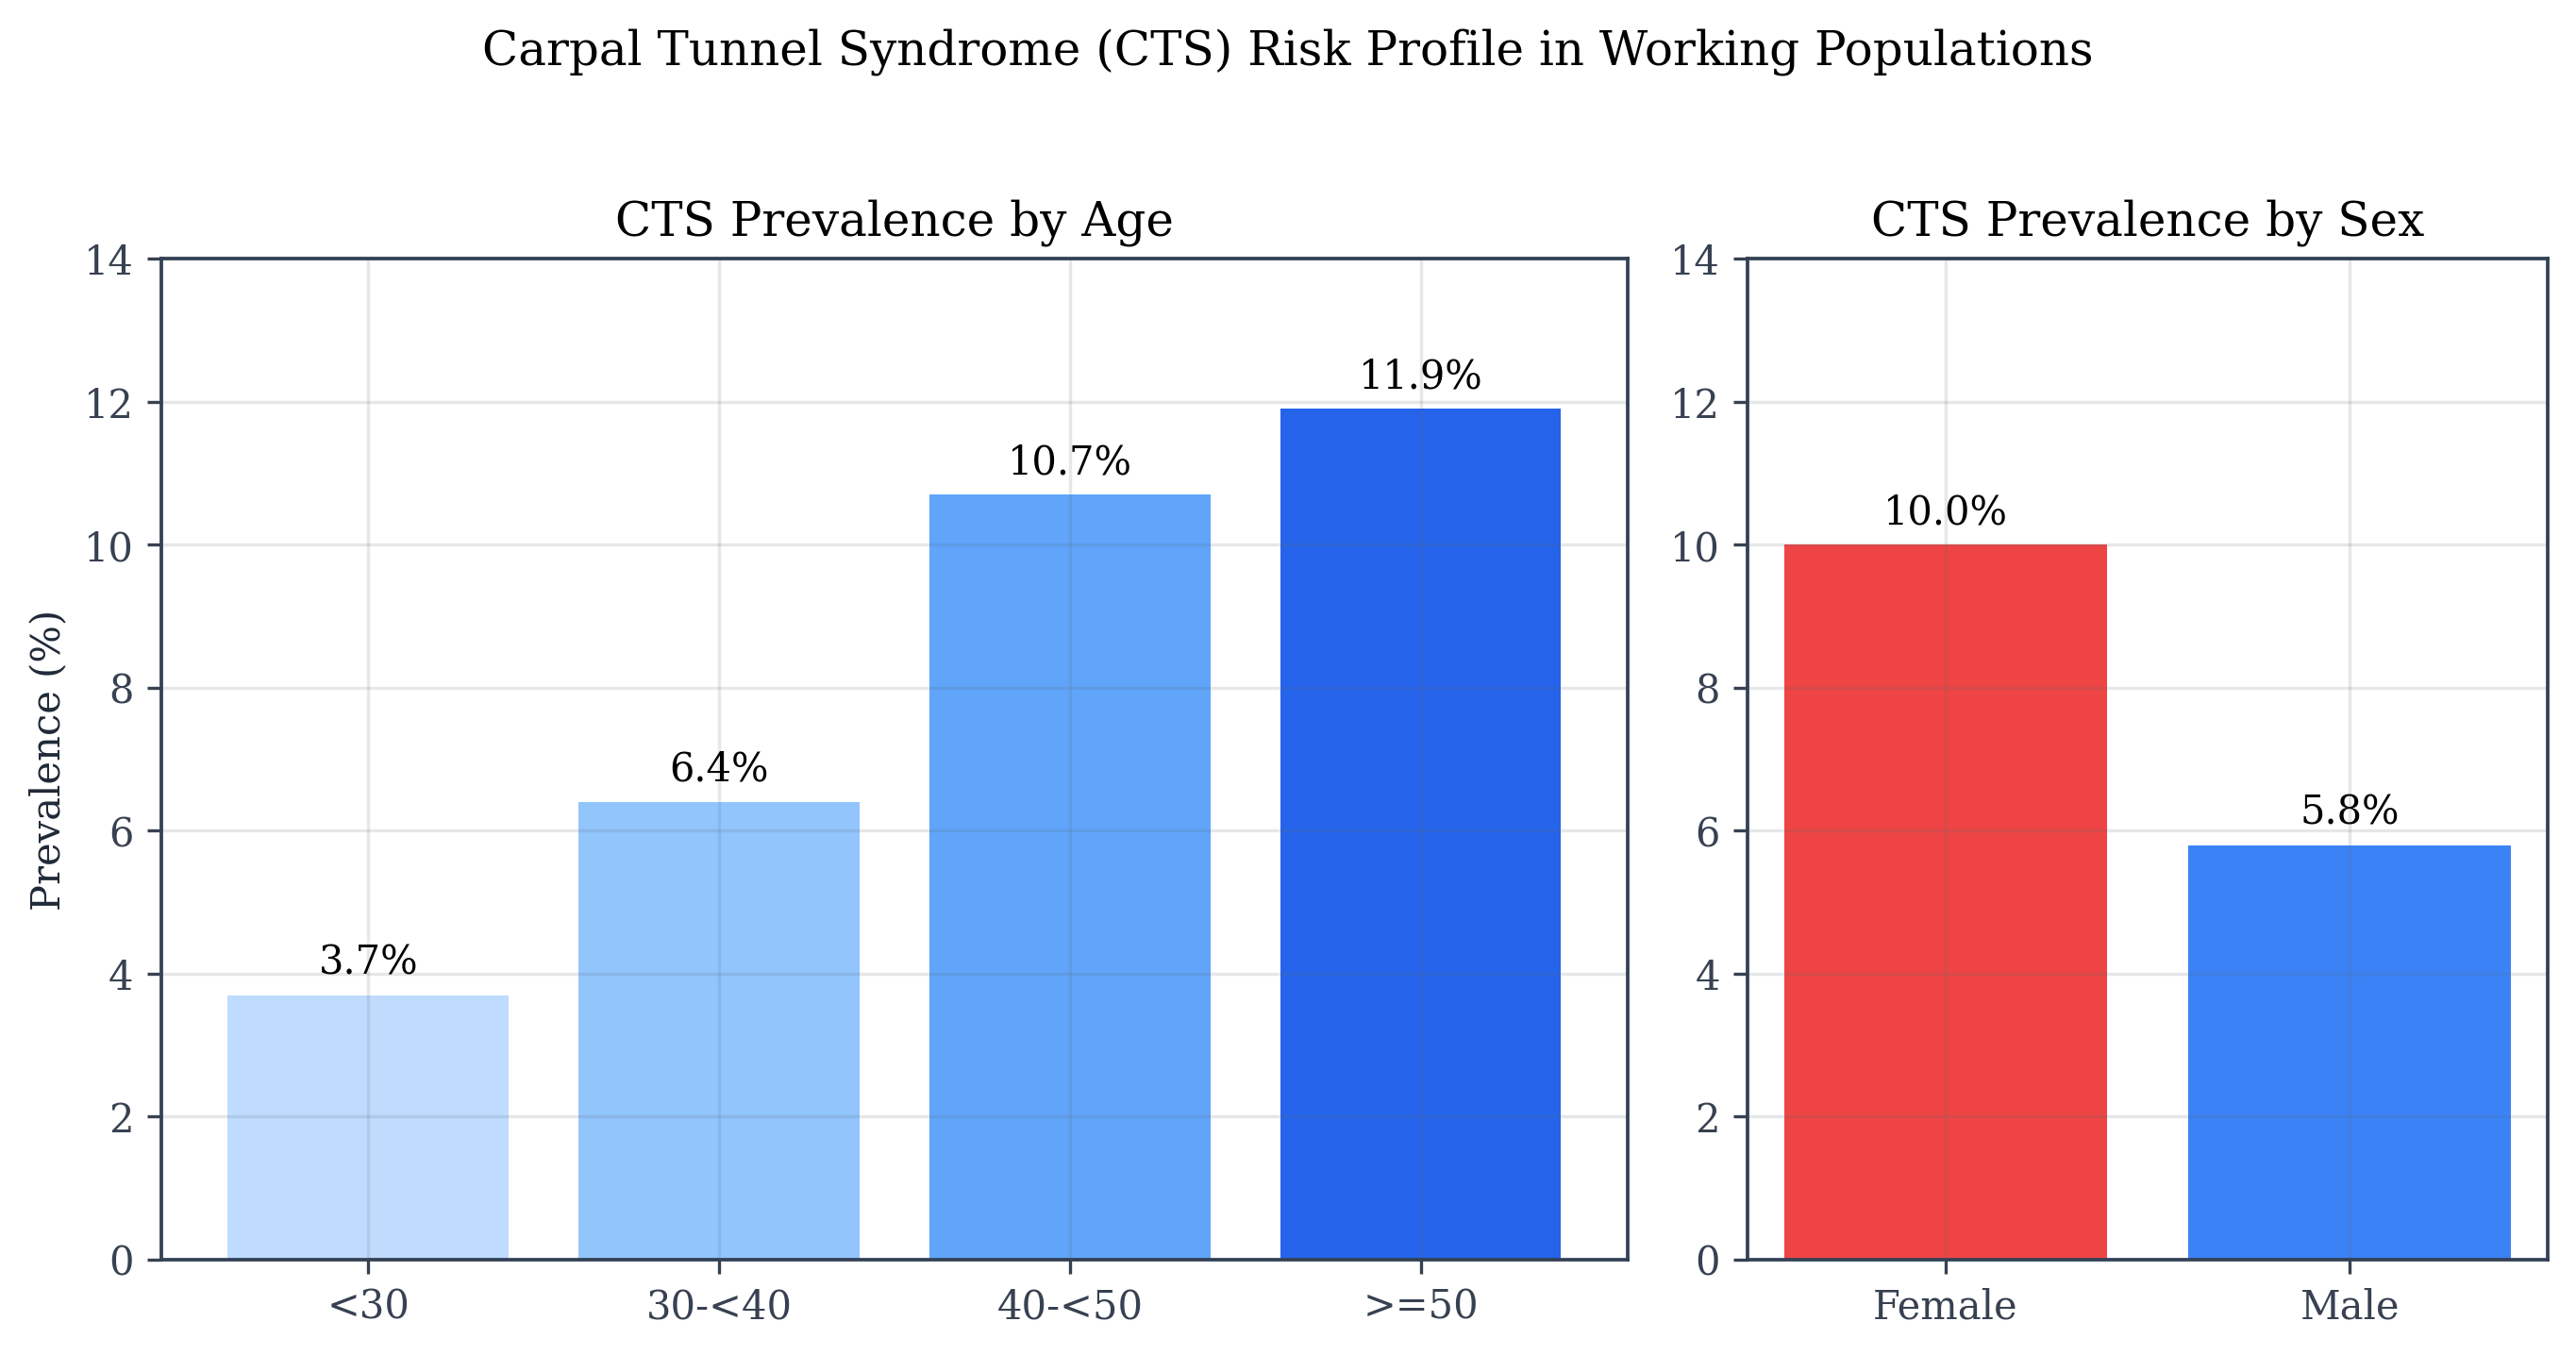
\includegraphics[width=0.7\linewidth]{img/ch1_cts_risk_profile.png}
  \caption{CTS Prevalence Profile by Age and Sex in Working Populations}
  \label{fig:cts_risk_profile}
\end{figure}

CTS burden is also patterned by demographic factors, with higher prevalence in older age groups and among female workers, as shown in Figure~\ref{fig:cts_risk_profile}. This distribution supports prioritising high-exposure and clinically vulnerable user segments in problem framing.

The profile indicates that occupational risk is not uniformly distributed and should be interpreted with exposure conditions, age structure, and workforce composition in mind. This supports prioritising high-intensity computer-use settings and user groups with elevated baseline vulnerability during requirements framing.

Exposure-time findings reinforce the clinical concern. Mouse use above 50\% of work time is associated with significantly higher odds of hand and wrist symptoms~\cite{andersen2003mouse}, and prolonged weekly exposure is linked to forearm pain risk~\cite{thomsen2008mouse}. For carpal tunnel syndrome (CTS), pooled occupational data report 7.8\% prevalence and an incidence rate of 2.3 cases per 100 person-years~\cite{dale2013cts}. Subclinical effects precede formal diagnosis: one study identified electrophysiological median-nerve entrapment in 34.8\% of asymptomatic long-term mouse users~\cite{ali2010median}.

\subsubsection{Accessibility Mismatch and Exclusion Risk}

The classical pointer-click paradigm presumes stable fine-motor control for both trajectory correction and click stabilisation. This assumption excludes many users with tremor, weakness, pain, or motor variability. The affected population is large: osteoarthritis alone affects approximately 595~million people globally~\cite{gbd2023oa}, and significant prevalence is documented across essential tremor~\cite{zheng2021essential}, cerebral palsy~\cite{mcintyre2022cp}, Parkinson's disease~\cite{maserejian2020parkinson}, and multiple sclerosis populations~\cite{lamers2016upperlimb}.

Empirical human-computer interaction (HCI) research identifies specific breakdown points in classical mouse interaction for motor-impaired users: precise target acquisition and click activation without cursor displacement~\cite{wobbrock2008goal}. In arthritis cohorts, 85\% of participants reported computer-use difficulties at considerable or very high levels~\cite{baker2009arthritis}. At societal level, these barriers align with observed digital-access disparities, including substantially lower device ownership rates among adults with disabilities~\cite{perrin2021disabilitytech}.

\subsubsection{Environmental Dependency and Contextual Inflexibility}

Classical mouse and trackpad systems are architecturally surface-dependent. Effective operation assumes access to a flat, stable workspace and a body posture compatible with sustained planar hand motion. This surface-availability assumption fails in many real-world use contexts, including standing presentations, bedside interaction, fieldwork, and ad hoc mobile workstations. The consequence is a contextual mismatch: computing is increasingly ubiquitous, yet primary input tools remain optimised for fixed-desk environments and cannot follow users into contexts where such environments are unavailable. This limitation is particularly relevant for the use cases that motivate the present work, where surface-independent, posture-flexible input is a core requirement.

\subsubsection{Interaction-Bandwidth Constraint}

Beyond health and accessibility, classical pointing interaction imposes a representational bottleneck by mapping rich hand-arm movement onto two-dimensional surface translation. Comparative pointing-performance studies have shown that gyroscopic spatial input currently trails mouse throughput, but remains functionally competitive and technically improvable~\cite{ramcharitar2017fitts}. This indicates that the problem is not an absence of alternatives, but the absence of an approach that jointly optimises ergonomics, accessibility, portability, and precision.

\begin{figure}[!hb]
  \centering
  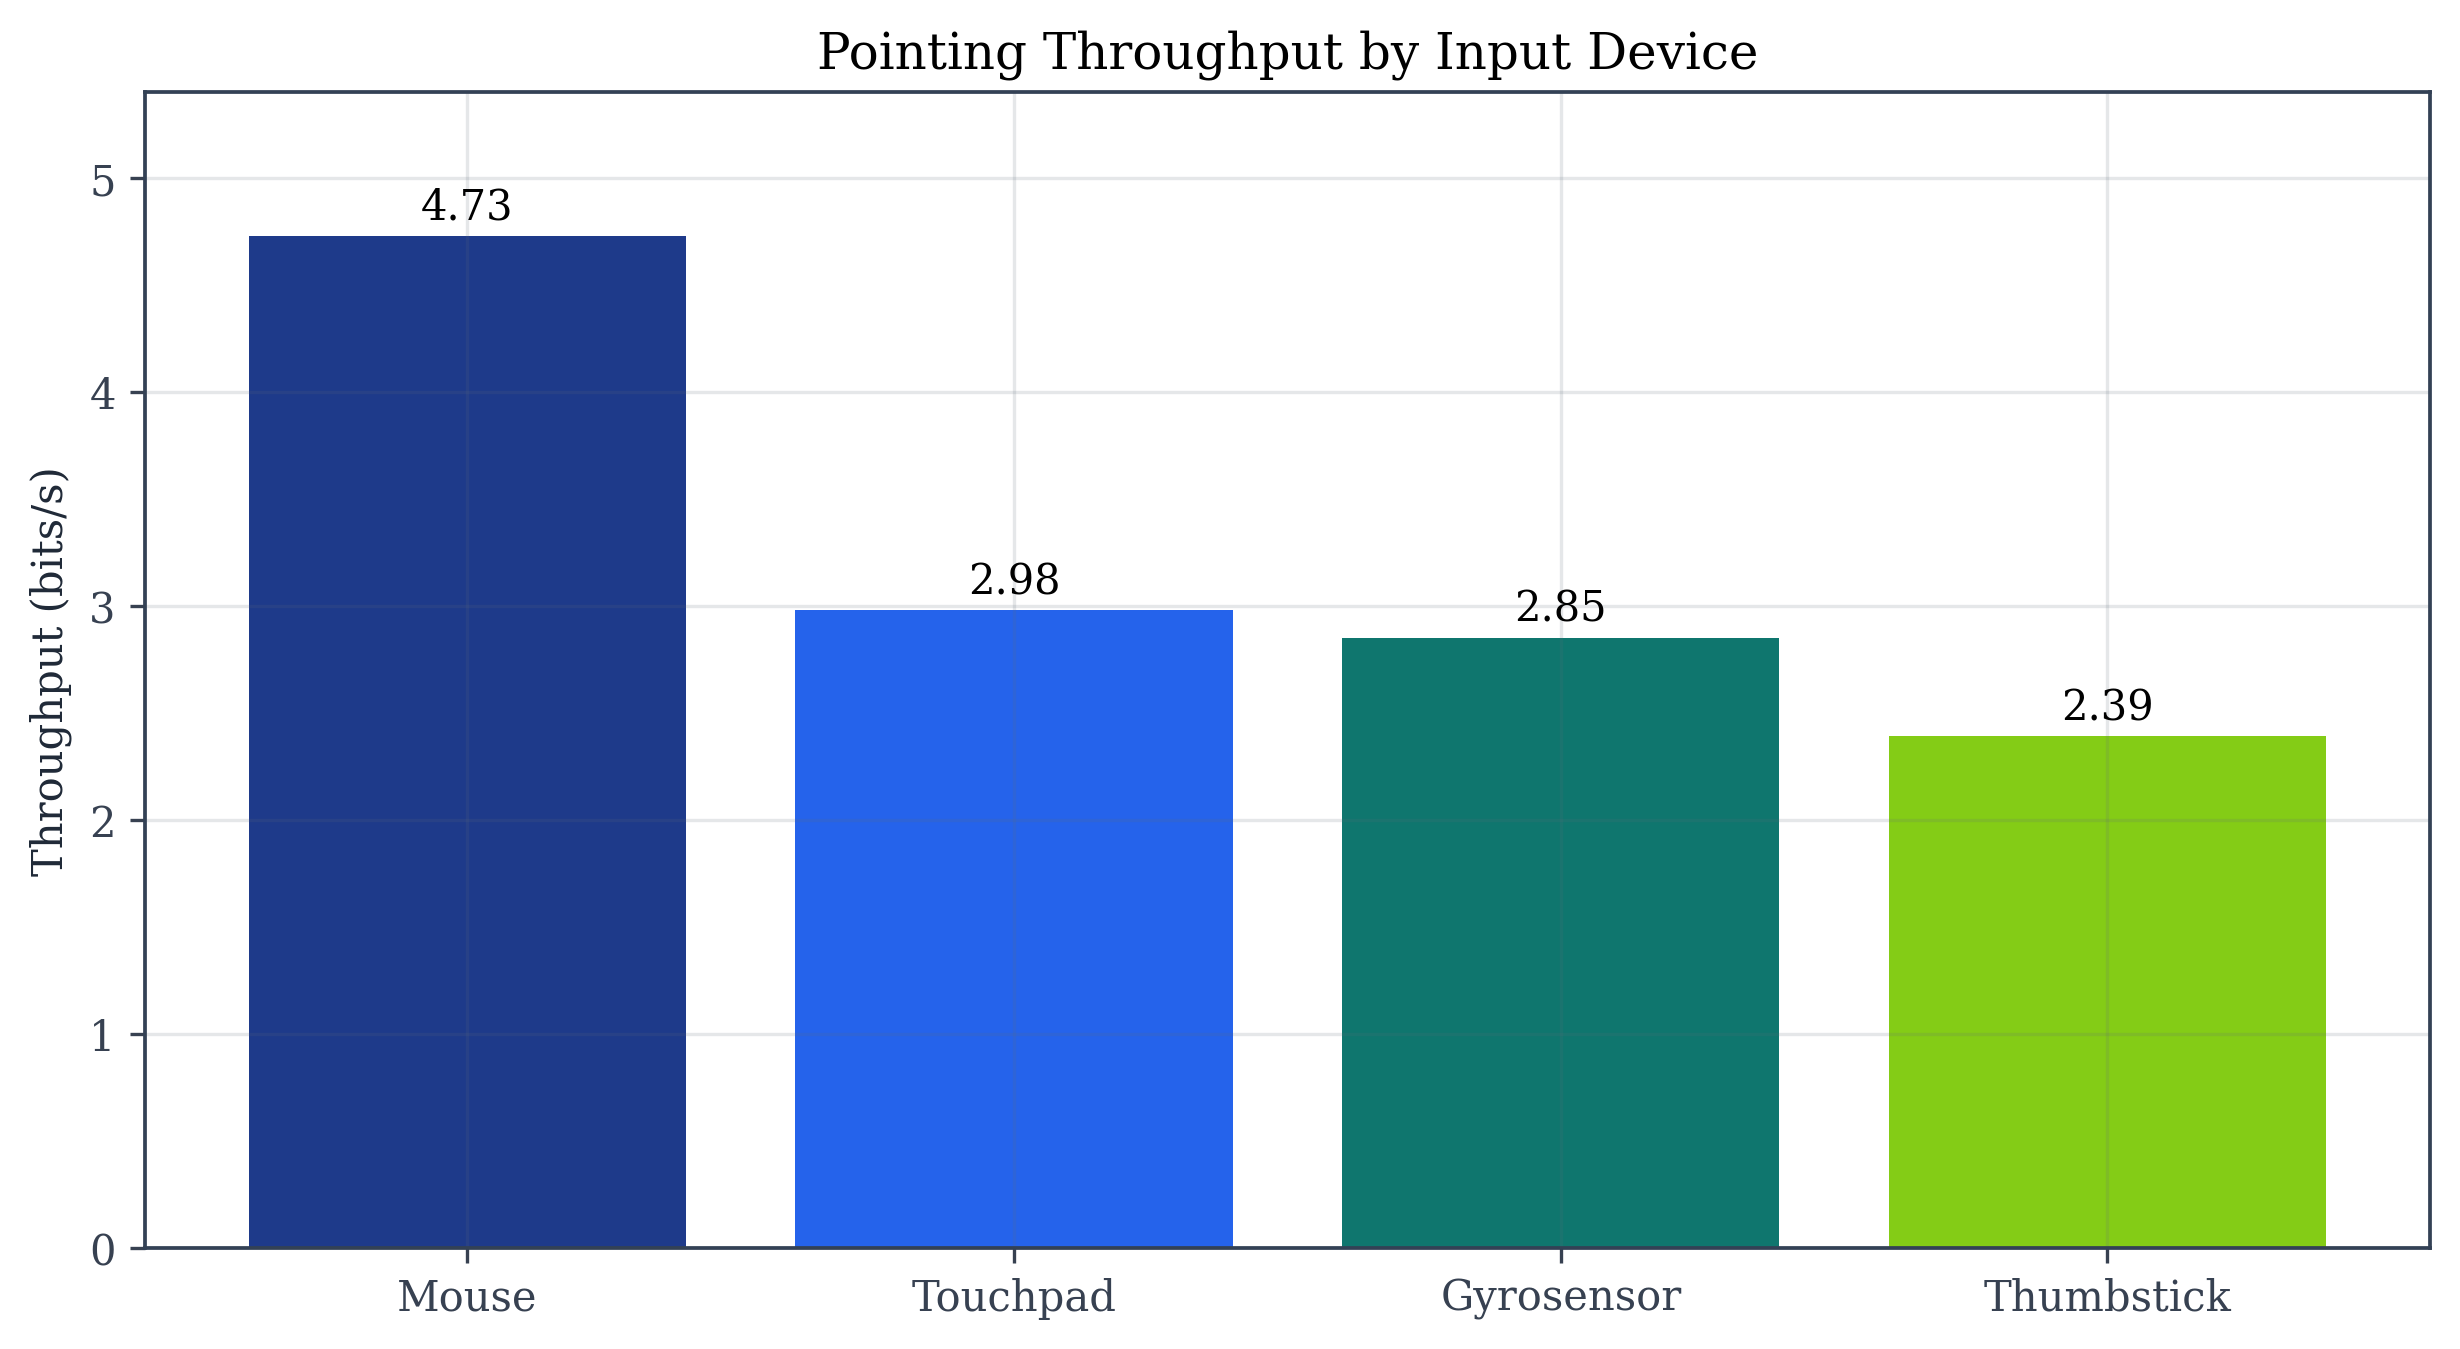
\includegraphics[width=0.7\linewidth]{img/ch1_input_throughput_comparison.png}
  \caption{Pointing Throughput Comparison Across Input Devices}
  \label{fig:throughput_comparison}
\end{figure}

Figure~\ref{fig:throughput_comparison} presents the reference throughput comparison used in this chapter and clarifies the current performance gap that motivates algorithmic and interaction-design refinement. Although the throughput gap remains meaningful, the comparison still positions gyroscopic interaction above some conventional controller modalities. This supports treating performance as an optimisation target rather than a hard feasibility barrier.

Appendix Table~\ref{tbl:problem_indicators} presents key quantitative indicators used to delineate the problem space and justify investigation of alternative input approaches. Taken together, these indicators justify the present work as a problem-driven intervention rather than a novelty-driven interface variant.

Following the above analysis, the following problem statement has been derived: Classical mouse- and trackpad-based interaction imposes cumulative biomechanical strain, depends on fixed planar workspaces, and inadequately accommodates motor variability across the user population, creating a demonstrable need for a wearable, movement-native input approach that improves ergonomic sustainability and accessibility while preserving functional pointing performance.
